\documentclass[10pt]{beamer}

\usetheme[progressbar=frametitle, numbering=fraction,]{metropolis}

\usepackage{booktabs}
\usepackage{pgfplots}
\usepgfplotslibrary{dateplot}
\usepackage{texshade}      
\usepackage{amsmath}
\usepackage{amssymb}
\usepackage{xspace}
\usepackage{xcolor}
\usepackage{appendixnumberbeamer}
\usepackage{multirow}


  
\newcommand{\themename}{\textbf{\textsc{metropolis}}\xspace}

\setbeamercovered{invisible}
\setbeamertemplate{caption}{\raggedright\insertcaption\par}

\title{ Controlling for conservation in genome-wide DNA methylation studies}
%: \textit{Evolutionary} Ideas}
\subtitle{M. Singer and L. Pachter, BMC Genomics(2015)}
\date{\today}
\author{Saket Choudhary}
%\institute{Center for modern beamer themes}
%\titlegraphic{\hfill
\includegraphics[height=1.5cm]{logo}}

\begin{document}

\maketitle

%\begin{frame}{Table of contents}
%  \setbeamertemplate{section in toc}[sections numbered]
%  \tableofcontents[hideallsubsections]
%\end{frame}

\begin{frame}[fragile]{DNA Methylation}
\begin{itemize}
\item Either cytosine(C) or adenine(A) undergoes methylation
\item Typically represses gene expression
\item Typically occurs in a `CpG' context (C followed by G)
\item Methylated C often deaminates to T
\end{itemize}
\end{frame}

\begin{frame}[fragile]{Yule-Simpson Effect: Example from University Admission}
\footnotesize
 %\begin{columns}[T,onlytextwidth]
    %\column{0.3\textwidth}
    \begin{center}
    \begin{table}
    \begin{tabular}{|c|c|c|}
    \hline
    & Female & Male\\
    \hline
    Applicants & 550 & 550 \\
    \hline 
    Admitted & 28.2\% & 41.8\% \\
    \hline
    \end{tabular}
    \caption{Acceptance percentage of female candidates is far less}
    \end{table}
    \end{center}
    \begin{center}
	\uncover<2->{\footnotesize
    \begin{table}
\begin{tabular}{|c|c|c|c|c|}
\hline
\multirow{3}{*}{} & \multicolumn{2}{|c|}{Female} &  \multicolumn{2}{|c|}{Male}\\
\cline{2-5}
& Applicants & Admitted & Applicants & Admitted\\
\cline{2-5}
Department A & 150 & 50\% & 400 & 50\%\\
\hline
Department B & 400 & 20\% & 150 & 20\%\\
\cline{1-5}
\end{tabular}
\caption{Departments do not display gender specific bias. Lower admission rates in female arises due females applying to department which are `harder' to get into}
\end{table}
    }
    \end{center}
\end{frame}

\begin{frame}[fragile]{Yule-Simpson Effect: Averaging methylation states can be misleading}
\begin{figure}
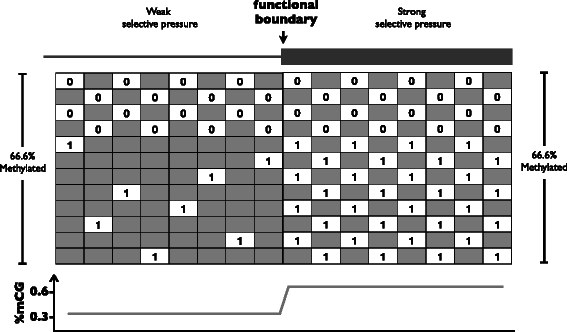
\includegraphics[width=\textwidth]{img/ys-boundary}
\caption{There is NO difference in methylation levels. YS Effect: Low frequency of methylated CGs in the left matrix}
\end{figure}
\end{frame}


\begin{frame}[fragile]{Yule-Simpson Effect: Geometric Interpretation}
\begin{figure}
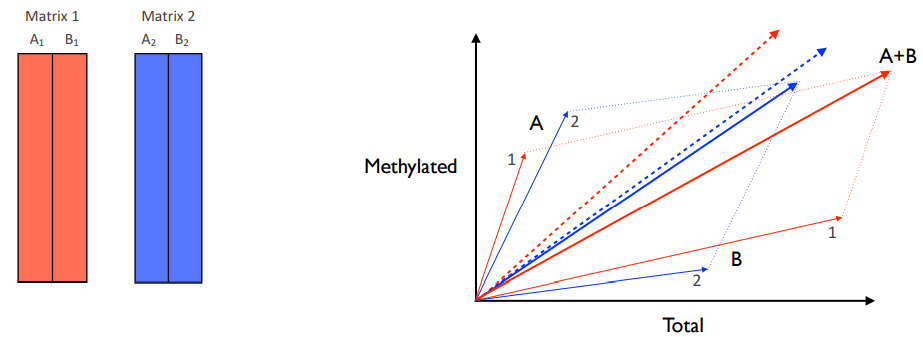
\includegraphics[width=\textwidth]{img/geometric}
\caption{Average of the slopes is reverse of the slopes of average}
\end{figure}
\end{frame}


\begin{frame}[fragile]{YS effect arises due to different rates of selection}
\begin{figure}
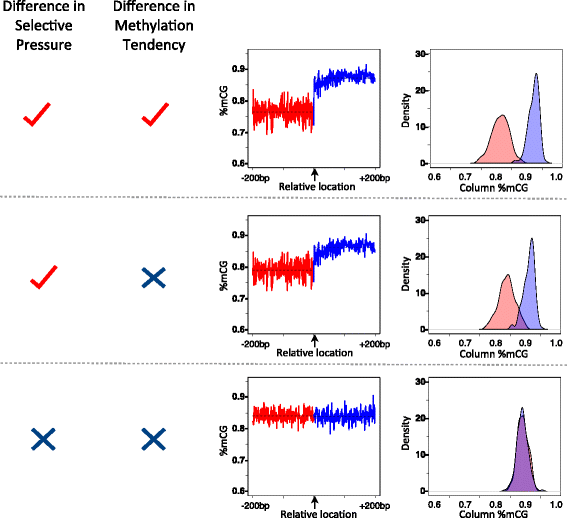
\includegraphics[scale=0.4]{img/fig2}
\caption{CpG = Missing data due to evolutionary constraint}
\end{figure}
\end{frame}

\begin{frame}[fragile]{Correction Method 1: Paired region averaging}
\begin{figure}
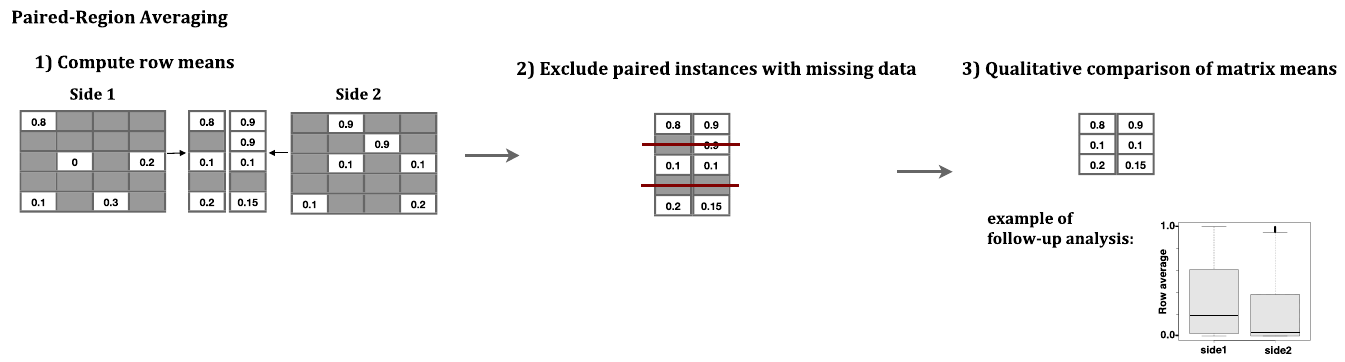
\includegraphics[scale=0.33]{img/method1}
\caption{Discarding data overcomes YS-effect. Only qualitative comparisons permitted}
\end{figure}
\end{frame}

\begin{frame}[fragile]{Correction Method 2: COMPARE (COMparison of
Phenotypes Averaged by REgion)}
\begin{figure}
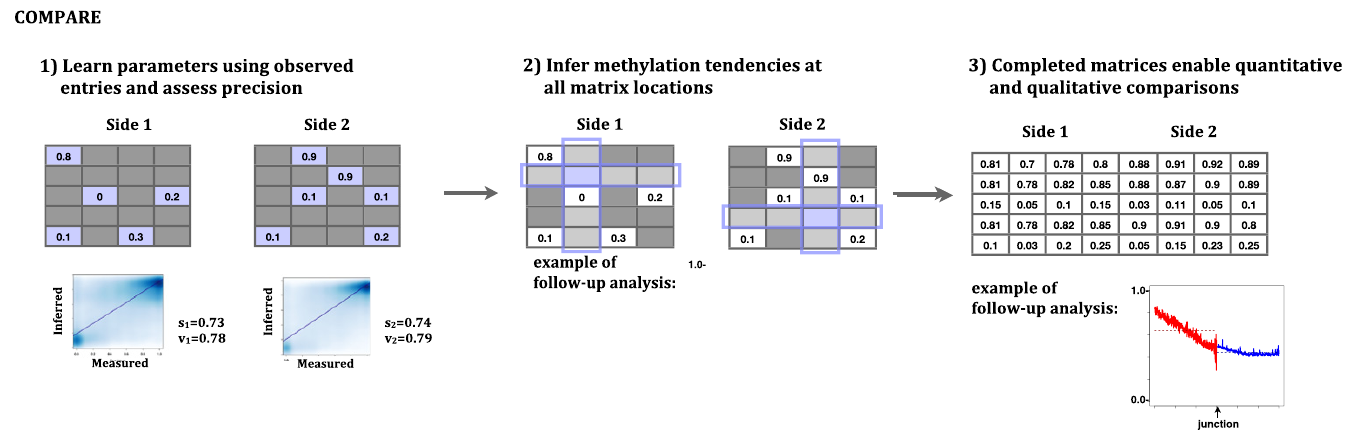
\includegraphics[width=\textwidth]{img/method2}
\end{figure}
\end{frame}

\begin{frame}[fragile]{Key findings}
\begin{figure}
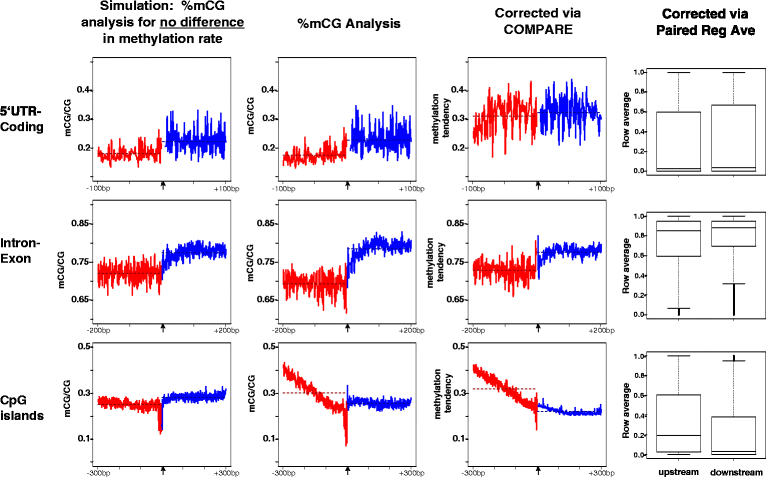
\includegraphics[width=\textwidth]{img/fig3}
\end{figure}
\end{frame}

\begin{frame}[fragile]{Key findings}
\begin{itemize}
\item Reanalysis of 5'UTR-coding boundaries revealed no significant difference in methylation tendencies
\item Intro-exon junctions in both human and Arabidopsis revealed difference in methylation levels
\end{itemize}
\end{frame}



\begin{frame}[fragile]{Correction Method 2: COMPARE (COMparison of
Phenotypes Averaged by REgion)}
\begin{align*}
M_{i,j} &= \frac{1}{1+e^{-(b_jB_{i,j}+x_jX_{i,j}+y_jY_{i,j}+z_j)}}\\
X_{i,j} &= \text{Mean(row i) excluding $(i,j)$ entry}\\
Y_{i,j} &= \text{Proportion of sites in row i with missing data}\\
B_{i,j} &= \text{Indicator variable for methylability}\\
b_j, x_j, y_j, z_j &= \text{Learned parameters}
\end{align*}
\end{frame}


\begin{frame}[fragile]{Summary}
\begin{itemize}
\item N\"{a}ive averaging approaches can be heavily biased due to non-uniformity of underlying distribution
\item Paired region averaging is a non-parametric approach that accounts for this non-uniformity for quanlitative comparison
\item COMPARE is a parametric approach allowing quantitative comparison between regions
\end{itemize}
\end{frame}


\end{document}
